\section{Approach}
\label{sec:Approach}

This section outlines the proposed approach, methodology and research gaps currently existing for each subproblem. A solution to robust manipulation of articulated objects consists of perception and control algorithms designed to work together. The building blocks of the proposed approach build upon the following core components:
\begin{itemize}
\item closed-loop physics-aware control
\item affordances based perception
\item active model estimation und uncertainty reduction
\end{itemize}
In the rest of this section, an overview of the methodology, underlying assumptions and a description of each subgoal are provided. 

\paragraph{Methodology} Each proposed solution is first evaluated in simulation and then on the real hardware consisting of the Royal-Panda mobile manipulator platform. The robot consists of a 7-DoF Franka Emika arm mountend on the holonomic Clearpath Ridgeback base. 

\paragraph{Assumptions} In this research plan the following assumptions are made:
\begin{itemize}
\item the object category is recognized prior to manipulation
\item manipulation can be solved in a non-prehensile manner: grasping is not required
\item sensing modalities are RGB-D images, point clouds, proprioceptive data and wrist-mounted wrench measurements 
\item articulated objects are restricted to the class of open loop kinematic chains consisting of a combination of revolute and/or prismatic joints
\end{itemize} 

\paragraph{Leveraging simulation} We believe that the potential of simulation engines (both for physical interaction and rendering) has not been fully exploited in the current research. Nevertheless, contemporary simulators are fast and accurate enough to replace analytical model while rendering engine afford photorealistic results. Recent behavioral and computation studies of human physical scene understanding push forward an account that people's judjement are best explained as probabilistic simulations of a realistic, but noisy physics engine~\cite{wu2015galileo}.
They can not only be used for offline synthesis and validation but also to generate manipulation behaviors and robust perception in real-time. The real-time offers the following advantages:
\begin{itemize}
\item Closed-loop control keep small the deviation of the simulation from the current observed state
\item The improved real-time estimate of model parameters (e.g joints' position and orientation) can be dynamically changed in the simulation
\item Detection algorithms can directly act in a virtual rendered scene which replicate the current simulated environment zeroing the \emph{sim-to-real} gap.
\end{itemize}
On the other hand, a full-scene simulation and rendering is computationally expensive. Therefore it is of utmost importance to come up with new algorithmic solutions that require little data or can cope with limited computational resources. As an example, one could decide to focus perception only on the object to be interacted with and reduce collision checks to the hand (gripper) and the few interaction points.  

\marginpar{
\begin{itemize}
	\item \emph{What approach will be used?}
	\item \emph{Why is the approach promising?}
	\item \emph{What are the expected results?}
\end{itemize}
}

\begin{figure}[h]
\centering
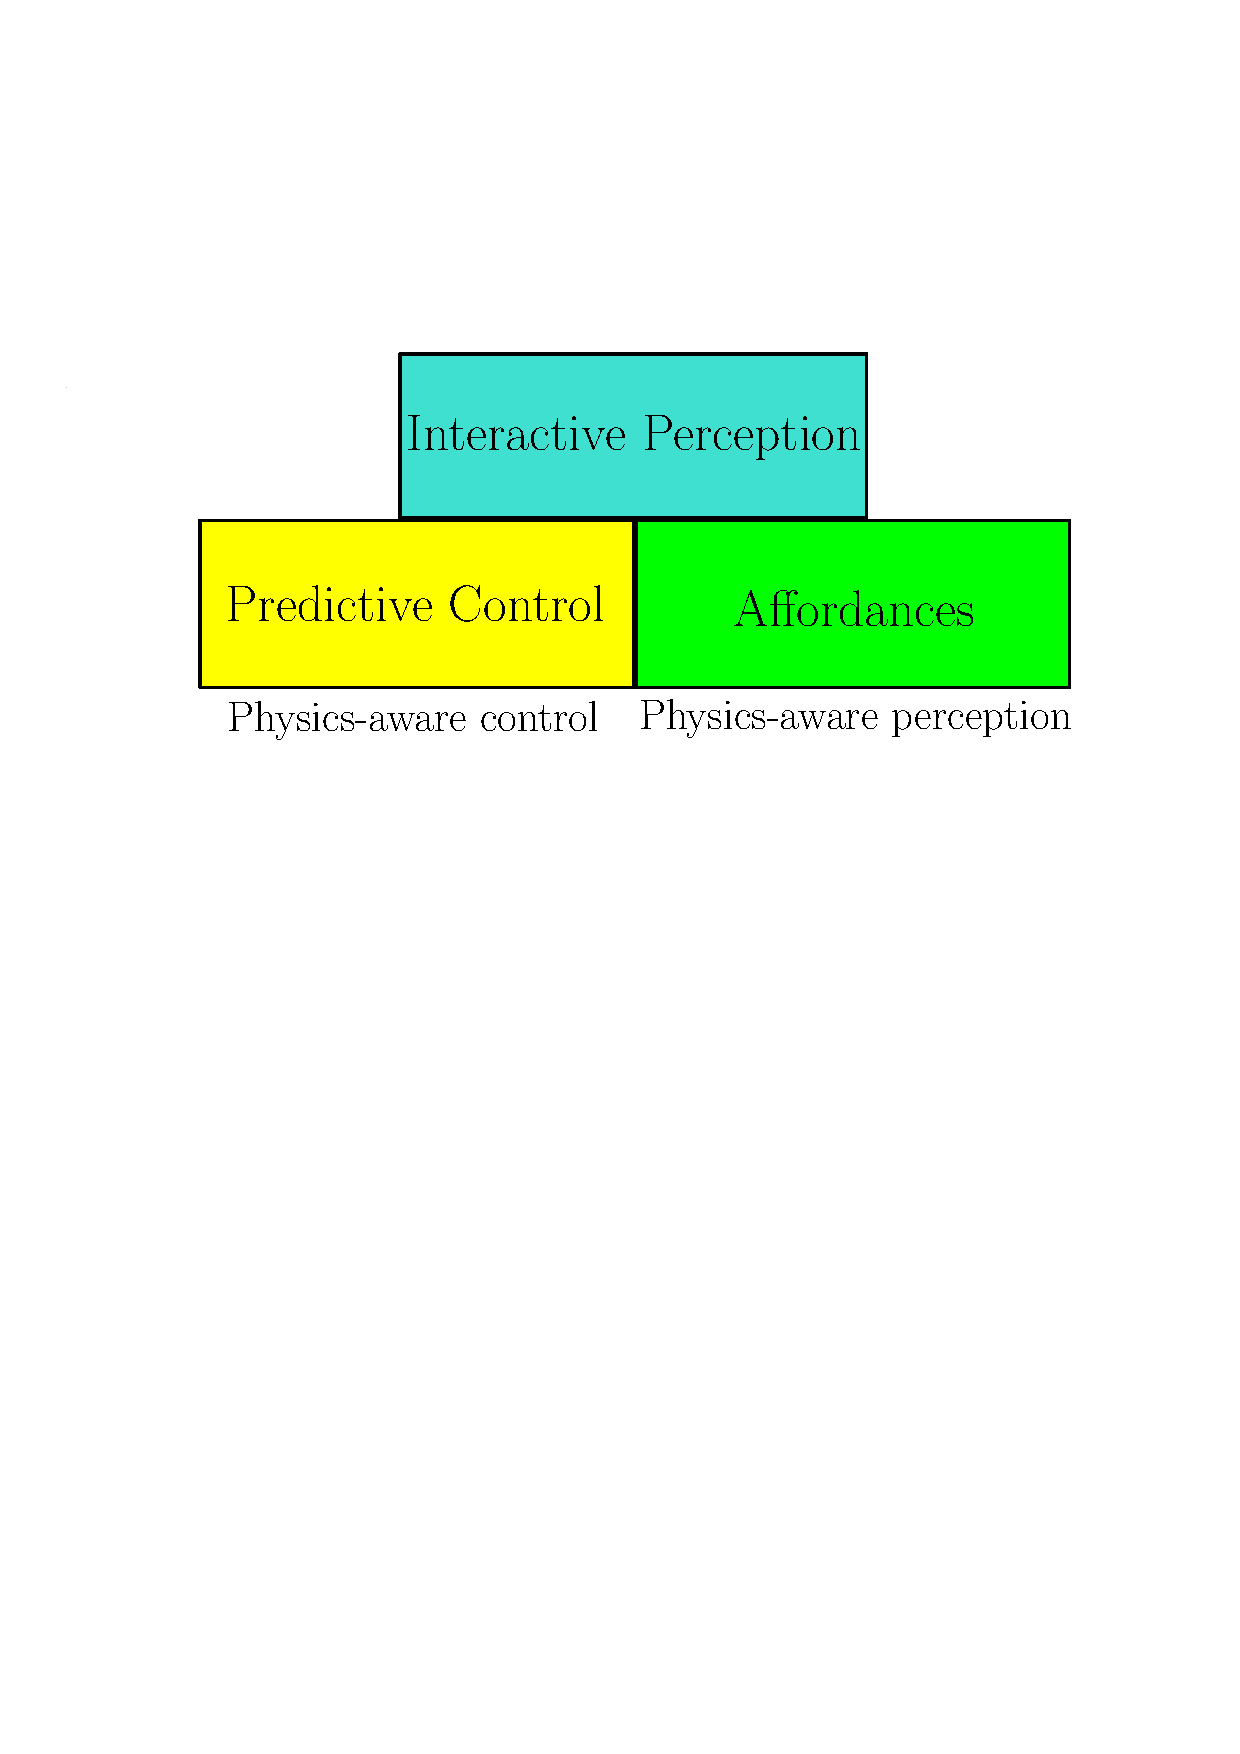
\includegraphics[width=0.6\textwidth]{images/blocks.pdf}
\caption{Building blocks of the proposed approach: \ldots}
\end{figure}

\subsection{Predictive Control}
The literature generally distinguishes between planning and control algorithms. In this research proposal control is the process of genereting a reference signal that the robot can track and brings the system's state (robot and object) to the desired one. A typical example is a velocity-controlled manipulator which has to open a door. A control algorithm is then in charge of generating the sequence of velocity values that allows the robot to interact with the door and move it to the open state. This definition is general enough to encompass various approaches. The velocity, for example, can be tracked by another low-level controller which compensates for gravity and Coriolis effects and commands robot torques. The controller could be split into an intermediate step where a reference end-effector trajectory is computed and this is then converted to low-level velocity signals. The proposed approach consists in planning directly in the joint velocity space as this allows to consider additional objectives such as joint limits and self-collisions. Furthermore, a low-level control layer which converts velocity references to torques is always used. In fact, tuning the low-level PD gains let us define a desired compliant behavior avoiding high interaction wrenches with the stiff environment. 
A cost function is then used as a proxy to inform the controller about the completeness of the task. In the running example, this could be the squared distance from the current door's joint angle to the one corresponding to the open position. 
Directly optimizing such a cost in the robot action space is extremely complex. In fact, the mapping between the optimization variables (velocities) and the cost is highly non-linear. The mapping goes through the full whole body dynamics and switching interactions that happen between the robot and the door. For this reason, we resort to gradient free methods. They come at the cost of being less sample efficient compared to gradient-based methods. Gradient-free methods rely on sampling input-state trajectories in simulation in order to drive the system towards optimality (see Sec.~\ref{sec:related_work_control}).

\subsubsection{Research gap and relation to previous works}
Using a fully fledged simulation backend exploits the fact that basic physcial concepts (e.g, distinct objects cannot occupy the same space, gravity applies mass-dependent force on objects, friction and kinematic constraints) provide strong prior knowledge for manipulation tasks~\cite{kroemer2019review}. In this first part of the work a practical receding horizon algorithm that achieves real-time whole-body control of a mobile manipulator using only a laptop CPU is proposed. This work is based on Model Predictive Path Integral control (MPPI)~\cite{williams_information_2017}, which is the underlying sampling-based controller for whole-body coordination and control. Several algorithmic elements enable the controller to achieve performant results, often requiring fewer than 100 rollouts. The main contribution is a regularization of our sampling exploration by means of a momentum update. This is inspired by the Bayesian inference viewpoint of~\cite{lambert_stein_2020}, which showes that the choice of exploration noise has the effect of tuning the gradient step size of the path integral update. The benefits of this sampling scheme are twofold, it can aid in escaping local minima while also damping strong oscillations in the optimal policy. Raisim phisics engine is used for fast and accurate simulation~\cite{raisim} while the pinocchio library~\cite{pinocchioweb} is used for rigid body dynamics modeling. The goal of this subtask is to verity the following hypothesis
\begin{displayquote}
\textit{Gradient-free methods are applicable with limited resources and in real-time for whole body mobile manipulation on a real platform.}
\end{displayquote}

\subsection{Results}
The developed algorithm is able to control a complex system in real-time without the need for massive parallel computation. To demonstrate the applicability and effectiveness of this approach, several ablation studies are performed in simulation on kinematic and dynamical manipulators. The full algorithm is then deployed on the \textit{RoyalPanda} platform for a target reaching and door opening task. An open source implementation of the solution is readily available at \url{https://git.io/Jtda7}. The results support the original hypothesis and encourage to deploy the algorithm to more challenging systems such as aerial vehicles.

\subsection{Affordances}
As mentioned in the previous section, control requires a reward signal to know which states are closer to the target state. In practice, the true objective is to manipulate the object to a target configuration but we do not care too much about the intermediate robot and object states. The cost then is generally an educated guess about this reward signal and can generally impose a structure not needed or even subpotimal for the manipulation problem. Consider the problem of turning a handwheel valve. The final objective (valve being turned) can be achieved in several different ways. For example one could grasp the wheel from the side or just apply a tangential push force to the ribs that connect the wheel to the shaft. It is argued here that designing a cost function that enforce a preference for one or the other approach is suboptimal for autonomous manipulation. Instead, the cost could be related to the concept of \emph{affordances}. The controller can then be informed about more generic interesting interaction regions.

\subsubsection{Research gap and relation to previous works}
The concept of \emph{affordances} for manipulation has been explored in many recent perception works. They mainly differ in the representation of object affordace as interaction points~\cite{gao2021kpam}, interaction regions~\cite{nagarajan2019grounded} or dense interaction likelihood and orientation maps~\cite{mo2021where2act}. Most of these works do not highlight the importance and applicability of the resulting perception pipeline for manipulation control. Furthermore an agreement on what is the optimal representation of affordances for object manipulation is still missing. In this part of the research proposal the aim is to combine affordances with control. The goal of this subtask is to verity the following hypothesis
\begin{displayquote}
\textit{Affordances allow to better exploit the structure in manipulation tasks with respect to fixed manipulation strategies.}
\end{displayquote}
The controller can try to bring the robot close to \emph{high-affordance} points. Note that this task can be hard or even unfeasible for traditional gradient based methods, while the sampling based algorithm so far developed lends itself well to this objective. 
Furthermore, a novel concept of affordances will be explored, by introducing, for example haptic information. Intuitively, human do not only know by experience where to act on object but also how. The latest prior can be expressed in terms of interaction orientations and expected wrench profiles (e.g. pulling vs pushing force). The goal of this second part of the project is to verify the following research hypothesis
\begin{displayquote}
\textit{Affordances describing haptic information are more descriptive then purely geometrical based affordances.}
\end{displayquote} 
In this task the SAPIEN simulators will be used since it integrates a comprehensive set of articulated objects normally found in households, provides ground truth segmentation and photo-realistic rendering~\cite{Xiang_2020_SAPIEN}. 

\subsection{Interactive Perception}
A fundamental aspect to take into consideration for object manipulation is model estimation and the associated \emph{hepistemic uncertainty} which is the uncertainty about the model parameters. For instance, we might not know the geometrical and physical properties of the object such as size, weight, friction, joint's position and orientation. Furthermore, uncertainty can be extened to other types of scene representations such as keypoints and interaction hotspots. Active perception will be investigated to reduce such uncertainty exploting the robot capacity to move sensors in space and changing the environment state. The concept of affordances developed in the previous section provides an information which is decoupled from the specific articulation model. If we are able to perceive which parts of the object are more likely to be interacted with and how, we are also imposing some prior on the type of the articulated object and viceversa. It is then possible to use affordances as a proxy for \emph{explorative actions} when the model is not available. In this part of the work the goal is to integrate interaction in the perceptive process. Forceful interaction, also known as \emph{peceptive manipulation}~\cite{bohg2017interactive} can be used to generate motion and information-rich signals and validate hypothesis about the articulation model. This validation can be performed in simulation which serves as a likelihood model. The plan is to integrate \emph{information seeking} actions in the developed stochastic control and perception framework. We assume that the object has been already categorized and a course estimate of the articulation model (category and model parameters) is available. The components so far developed will serve as building blocks of a simulataneous estimation and control pipeline which works in a closed-loop fashion. We will then investigate the following research hypothesis:
\begin{displayquote}
\textit{Simulation and affordance guided perceptive manipulation can cope with large uncertainty while simultaneously executing the task.} 
\end{displayquote}
The sensor modality used to develop the proposed algorithm will be RGB-D cameras and wrist mounted force torque sensors. End-effector mounted cameras are generally good for passive perception but unusable during manipulation because of heavy occlusions. Therefore, a shoulder or base mounted camera will be evaluated as additional sensory input.  
 
\subsubsection{Research gap and relation to previous works}
Object classification and articulation model estimation from visual data has been already addressed in previous works~\cite{he2017mask, li2020category}. Although showing promising results, the error from single-shot detection is still too large to deploy this estimate for modeling and control. The idea of refining the initial estimate using a physics engine to validate exploratory interactive actions has been investigated in~\cite{eppner2018physics}. The proposed method relies on a reactive sampling strategy and human intervention for an accurate initial estimate of the articulation model. Frequently, the grasp model is fixed as well the action parametrization. This assumptions restrict the type of possible interactions and the generalizability of the approach. Furthermore, methods generally split the problem of task excecution and model estimation~\cite{eppner2018physics}. Simultaneous parameter estimation and control has been not fully explored for manipulation tasks and has been only applied to small dimensional systems and low dimensional parameters' space~\cite{barcelos2021dual}. 